For excitation dominates ionisation, the loss of energy that is necessary to ionise an atom is
larger than the ionisation energy of the atom. The mean number of electron-ion-pairs is given by 

\[\frac{\text{Energieverlust des Teilchens}}{\text{mittlere Energie für die Erzeugung eines
$e^-$-Ion-Paares}} \]

Typical values for the required energy are about $30\,$eV. This way, a particle with $3\,$keV
produces about $\frac{3000\,\text{eV}}{30\,\text{eV}}=100$ $e^-$-ion-pairs.

\begin{figure}[H]
	\centering
	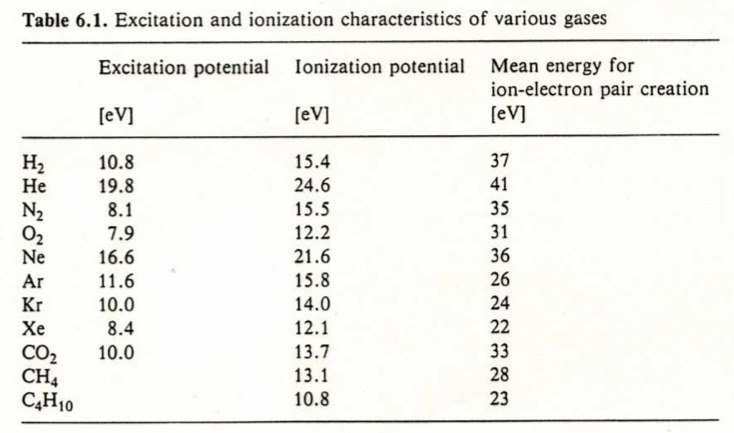
\includegraphics[width=0.5\textwidth]{Fig-03-01.jpg}
\end{figure}

The goal is to determine the loss of energy of particles. The idea is to count the number of the
produced $e^-$-ion-pairs - the larger the number, the more precise the measurement. 

\[\text{particle energy}\approx \#(\text{$e^-$-ion-pairs})\cdot (\text{mean energy for one
$e^-$-ion-pair})\]

For a number $N_{\text{Mess}}\ge 20$, we obtain a Gauss curve for repeated measurements of the
produced primary total ionisation.

\begin{figure}[H]
	\centering
	
\includegraphics[width=0.5\textwidth]{dummy.jpg}
\end{figure}

The relative resolution in this case is given by

\[\frac{\sigma_{a}}{\langle a \rangle} =
\frac{\sqrt{N_{\text{Mess}}}}{N_{\text{Mess}}}=\frac{1}{\sqrt{N_{\text{Mess}}}}
\]

as the best possible resolution for a highly statistical process. In fact, we obtain small values
around the so called Fano factor $F$:

\[ F:=\frac{\text{observed resolution}}{\text{expected resolution (from Poisson statistics)}} \]

Examples:

\ldots

The ionisation processes are not statistically independent!
